\documentclass[11pt, a4paper]{report}
\usepackage[utf8]{inputenc}

\usepackage{listings}
\usepackage[framed,numbered,autolinebreaks,useliterate]{mcode}

\usepackage[margin=1in]{geometry}
\usepackage{graphicx}
\usepackage{amsmath}
\usepackage{amsfonts}
\usepackage{float}
\graphicspath{ {images/} }
\setlength\parindent{0pt}


\newcommand{\p}{\partial}
\newcommand{\mth}[1]{
  \begin{align*}
    #1
  \end{align*}
}


\usepackage{appendix}
\usepackage{chngcntr}
\usepackage{etoolbox}
\usepackage{lipsum}

\newcommand{\newappendix}{%
  \refstepcounter{chapter}\chapter*{Appendix \thechapter}%
  \addcontentsline{toc}{chapter}{Appendix \thechapter}%
}

\begin{document}

\begin{center}
  \Huge Floppy Drive Orchestra \\
  \huge University of Colorado Boulder \\
  \Large Independent Study\\
  
  \vspace{6in}
    \huge Jeffery Lim \\
    \huge Jeffery.Lim@colorado.edu\\
    \Large Under supervision of Dr. Shalom Ruben \\~\\~\\
\end{center}
\pagebreak

\tableofcontents

\chapter{Introduction}

The goal of the floppy drive orchestra was to not only develop a working orchestra, but understand the data flow to allows music to be played from something that is used to read and write. 

\chapter{Floppy Drive Characteristics}

The first tests conducted were the analysis of a single floppy drive unit. Floppy drives come in three sizes: 8 in, 5.25 in, and 3.5 in. The large floppy drives come with different characteristics, however, the more modern 3.5 in floppy drive will be used.

\begin{figure}[H]
\hspace*{-2cm}    
    \centering
    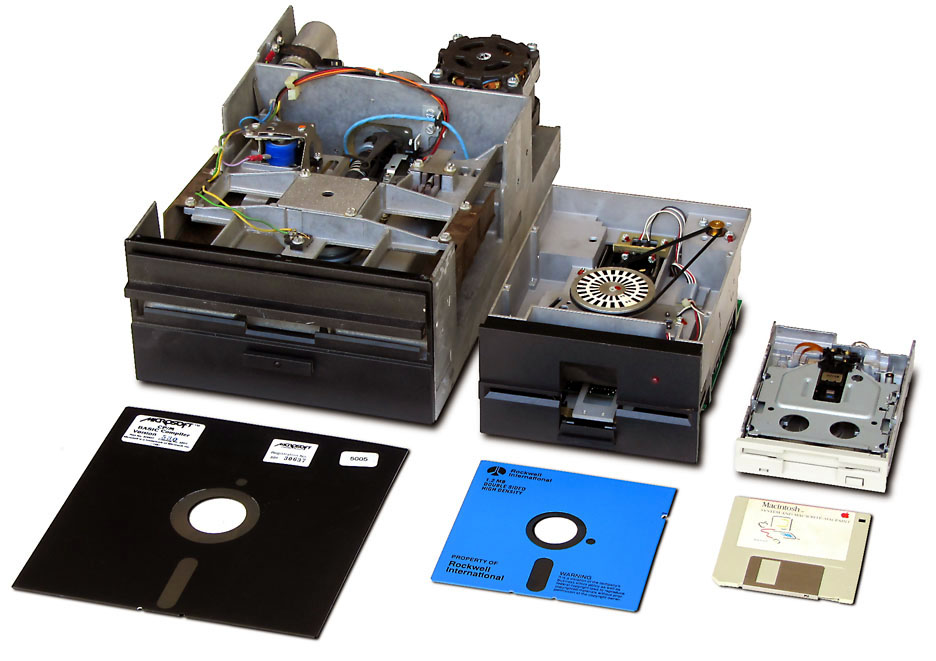
\includegraphics[width=.3\textwidth]{floppydrive_sizes.jpg}
    \caption{Floppy Drive of All Sizes}
    \label{fig:sizes}
\end{figure}

\section{Power}

The floppy drive takes a mini Molex cable as seen in Figure \ref{fig:miniMolex}. A mini Molex cable has a 5V line as well as 12V. Modern floppy drives used to use the 12V line for the drive motor, however, more modern floppy drives only use the 5V to drive the entire drive. \\

\begin{figure}[H]
\hspace*{-2cm}    
    \centering
    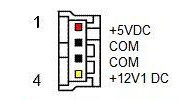
\includegraphics[width=.3\textwidth]{miniMolex.jpg}
    \caption{Floppy Drive Power Pinout}
    \label{fig:miniMolex}
\end{figure}


The power consumption of the drive when idling is an average of 50 mA and when the motor is active, it pulls 400 mA. \\


\section{Floppy Pinout}

The floppy pinout is shown in Figure \ref{fig:pinOut}. The bottom row, or the odd valued pins, are all grounded, where the top pins, or the even valued pins, are live. Each pin has a diferent functionality when it is grounded with the pins below. It is not necessary to connect the live pins to their respected ground pins, because the bottom row are all grounded. The actual names of the active pins are shown in Figure \ref{fig:pinNames}
\begin{figure}[H]
\hspace*{-2cm}    
    \centering
    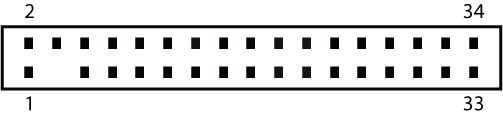
\includegraphics[width=.75\textwidth]{floppy_pinout.jpg}
    \caption{Floppy Drive Pinout}
    \label{fig:pinOut}
\end{figure}

\begin{figure}[H]
\hspace*{-2cm}    
    \centering
    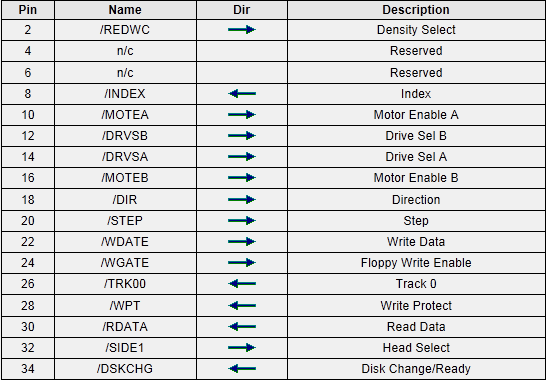
\includegraphics[width=.75\textwidth]{pinNames.png}
    \caption{Floppy Drive Pin Names}
    \label{fig:pinNames}
\end{figure}

The only necessary pins to drive the floppy drive motor head are pin number 12 or 14, 18, and 20. Pins 12 and 14 are the drive select B and A. These are the drive enable pins. Some drives are B drives and others are A, so in order to test them, either one of them will need to be sleected. These pins are equivalent to a drive enable.\\

Pin 18 is a direction pin. The direction is what determines the direction of the motor drive. When the pin is grounded, the drive heads moves away from the pins, and when the pin is high, the drive returns towards the pins. \\

Pin 20 is a step pin. This pin drives the stepper motor, so every time the pin goes high, the stepper motor will go forward one tick.\\

\section{Stepper Motor Movement}


\begin{figure}[H]
\hspace*{-2cm}    
    \centering
    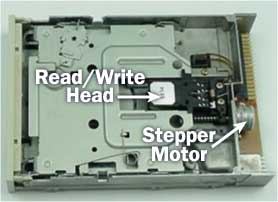
\includegraphics[width=.3\textwidth]{floppydrive_coveroff.jpg}
    \caption{Floppy Drive With Top Off}
    \label{fig:coveroff}
\end{figure}

The floppy drive motor head has a physical limit to how far it can go. To determine this value, a 1 Hz square wave is sent through to the floppy drive's direction pin (pin 18). The number of ticks is manually recorded. This can be run multiple times by simply disconnected or connecting the direction pin. \\

The total number of ticks a 3.5 in drive can go is 80, meaning the step pin (pin 20) needs to be toggled high 80 times before the drive reaches the limit. This means there needs to be a transition of high to low 80 times. Depending on the floppy drive, the motor will either continue to try and go forward, and others will not move. \\

\section{Stepper Motor Bandwidth}

Since the music will be played through the motor head, the bandwidth of the stepper motor will be a large limiting factor. For the test, a square wave from a waveform generator is connected to the step pin (pin 20), and the direction pin is connected to ground and disconnected in order to allow the motor head to switch direction. \\

The waveform generator is swepted from 1 Hz up until the motor head is no longer moving. The drive was able to handle up to 400 Hz, but afterwords, it was no longer consistent in terms of the speed of the drive. \\

This limit considerably restricts what the drive can play, and higher notes will need to be address. 



\chapter{Wiring Diagram}

Because the floppy drive only requires 5V and 400 mA each, there are two approaches in order to supply the power. A 5V power source with enough current to support all the drives is sufficient to power the system.
\section{Power}


As discussed in the previous chapter on floppy drive power characteristics, since each floppy drive, when running, draws 400 mA. For each floppy drive added to the system, the total power draw increases by 400 mA, so for 4 floppy drives, the total power consumption from the floppy drive system would be around 1600 mA, or 1.6 A. 
  
\section{Arduino Wiring}


\chapter{MIDI Files}

  MIDI, or Musical Instrument Digital Interface, is a standard that has its own protocols, interface, and connectors. It allows a single file to contain multiple tracks for several instruments in its own channel. This allows a MIDI file to play several instruments at once, up to a maximum of 16 instruments. This advantage of the MIDI file allows multiple floppy drives to be played at once, like how a MIDI file would send data to several instruments. 

\section{MIDI Notes}

The MIDI interface has notes that are mapped to specific piano keys at their respected frequencies. 
\begin{figure}[H]
\hspace*{-2cm}    
    \centering
    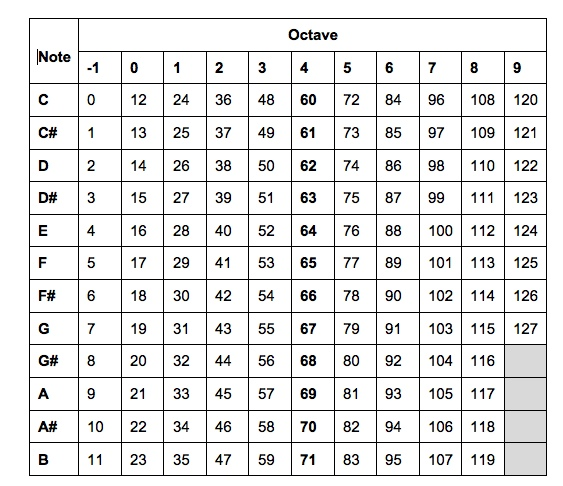
\includegraphics[width=.75\textwidth]{midi_notechart.jpg}
    \caption{MIDI Note Number to Key}
\end{figure}

\section{MIDI Messages}


\begin{center}
 \begin{tabular}{||c | c | c | c | c||} 
 \hline
  \multicolumn{5}{|c|}{MIDI Message} \\ 
 \hline\hline
  \multicolumn{3}{|c|}{Status}  & Data & Data \\
 \hline
  \multicolumn{2}{|c|} {Command (4 bits)} & Channel(4 bits)  & Note (8 bits) & Velocity (8 bits) \\
 \hline
  Note On & 1001 & nnnn  & 0xxxxxxx & 0vvvvvvv \\
 \hline  
  Note Off  & 1000 & nnnn  & 0xxxxxxx & 0vvvvvvv \\
 \hline
\end{tabular}
\end{center}

\chapter{Software}
\section{MIDI Player}
\section{MIDI to Serial Driver}
\section{Arduino}
\section{SD Card(?)}

\chapter{Arduino}
\section{Timer1 Library}
\section{Setup}
\section{Serial Reader}
\section{ISR}
\section{Floppy Drive Driver}
\section{SD Card(?)}


\pagebreak

\appendix
\newappendix\label{firstappendix}
\section{Full C Code}

\lstinputlisting[language=C]{../src/floppy/floppy.ino}

\end{document}
